\documentclass[a4paper, 12pt]{article}
\usepackage[a4paper, top=2.5cm, bottom=2.5cm, left=3cm, right=3cm]{geometry} %margenes
\usepackage[utf8]{inputenc} %manejo de caracteres especiales
\usepackage[spanish]{babel} %manejo de encabezados de inglés a español
\usepackage{fancyhdr} %formato de los encabezados de página
\usepackage{ragged2e} %alineado real justficado
\usepackage{graphicx} %manejo de imagenes
\usepackage{amsmath} %manejo de notación matemática
\usepackage{mathtools} %manejo de notación matemática
\usepackage{blindtext} %texto de relleno
\usepackage{amssymb} %manejo de simbología variada
\usepackage[titles]{tocloft} %manejo de elementos para el índice
\usepackage{float} %manejo de centrado para figuras
\usepackage{algorithm2e} %manejo de algoritmos
\usepackage{hyperref} %manejo d hipervínculos
\hypersetup{
    colorlinks=true,      
    urlcolor=blue,
    linkcolor=blue
}

\pagestyle{fancy}
\fancyhf{}
\rfoot{\thepage}

\begin{document}
    
    %PORTADA
    \begin{titlepage}
        \begin{figure}[ht]
            \centering
            
\includegraphics[width=15cm]{logosITT.png}
        \end{figure}
        \centering
        {\scshape\LARGE Tecnológico Nacional de México\\Instituto Tecnológico de Tijuana\par}
        \vspace{1cm}
        {\scshape\Large Investigación de Operaciones\par}
        \vspace{1cm}
        {\scshape\Large Unidad 3\par}
        \vspace{1.5cm}
        {\huge\bfseries Evidencias de ejercicios resueltos en C\# \par}
        \vspace{2cm}
        {\Large\itshape C. Abraham Jhared Flores Azcona,\,\# 19211640\par}
        \vfill
        Profesora: \par
        Ing. Igreyne Aracely Ruiz Romero
        
        \vfill

        {\large 19 de noviembre del 2020}
    \end{titlepage}

    \newpage
    \thispagestyle{empty}
    \tableofcontents
    \listoffigures

    \newpage
    \lhead{\textbf{Evidencias de ejercicios resueltos en C\#}}
    \section{Unidad 1}
    \subsection{Ejercicio 3}
    \begin{figure}[H]
        \[\begin{matrix}
            F\!.\!O:&\text{Max (z)}:&30x_1+40x_2\\
            S.\!a: &&x_1+x_2\leq 480\\
            &&x_1+2x_2\leq 800\\
            &&x_1,\,x_2\geq 0
        \end{matrix}\]
        \caption{Modelo del Ejercicio 3.}
    \end{figure}
    \begin{figure}[H]
        \centering
        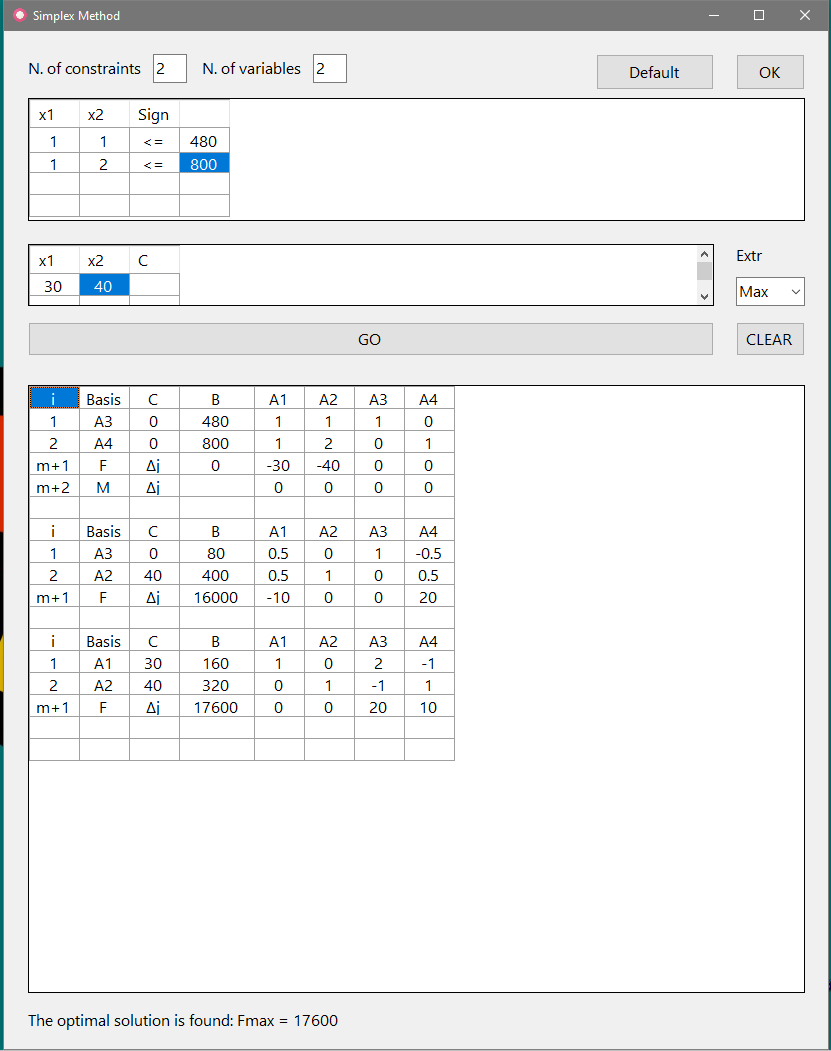
\includegraphics[width=12cm]{ejercicio3.PNG}
        \caption{Resolución del Ejercicio 3 en C\#.}
    \end{figure}
    \subsection{Ejercicio 4}
    \begin{figure}[H]
        \[\begin{matrix}
            F\!.\!O:&\text{Max (z)}:&50x+120y\\
            S.\!a: &&100x+200y\leq 10000\\
            &&10x+30y\leq 1200\\
            &&x+y\leq 110\\
            &&x,\, y\geq 0
        \end{matrix}\]
        \caption{Modelo del Ejercicio 4.}
    \end{figure}
    \begin{figure}[H]
        \centering
        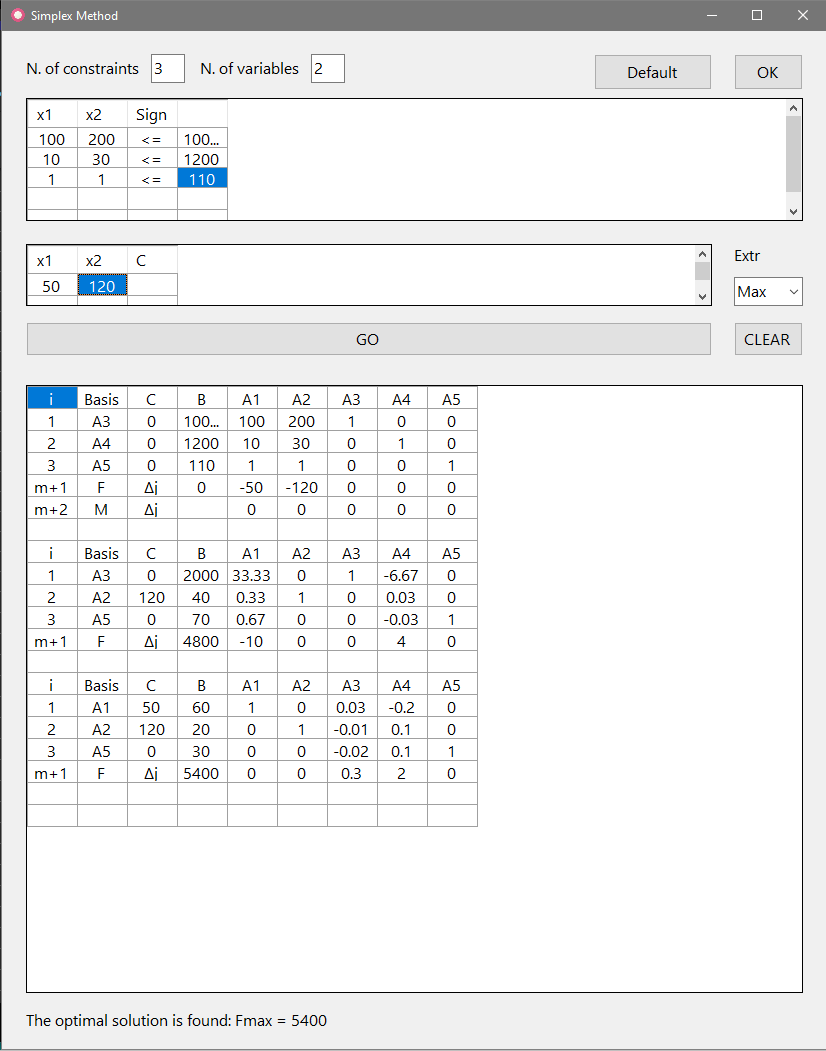
\includegraphics[width=12cm]{ejercicio4.PNG}
        \caption{Resolución del Ejercicio 4 en C\#.}
    \end{figure}
    \subsection{Ejercicio 5}
    El ejercicio resuelto es el mismo del Ejercicio 3.
    \subsection{Tarea 2}
    \begin{figure}[H]
        \[\begin{matrix}
            F\!.\!O:&\text{Max (z)}:&20000A+10000B\\
            S.\!a: &&2A+B\leq 10\\
            &&A+2B\leq 8\\
            &&A,\, B\geq 0
        \end{matrix}\]
        \caption{Modelo de la Tarea 2.}
    \end{figure}
    \begin{figure}[H]
        \centering
        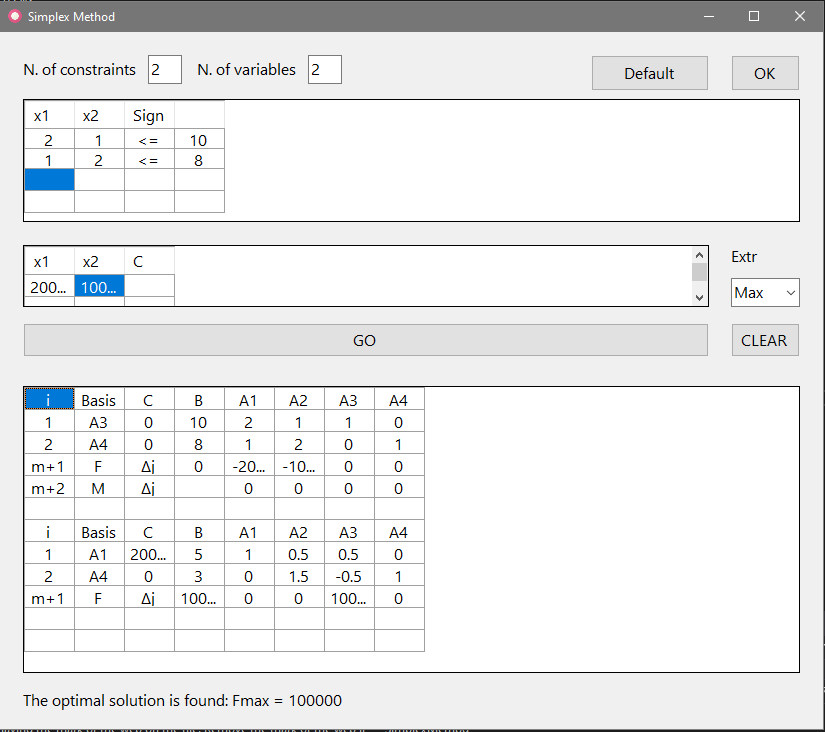
\includegraphics[width=12cm]{tarea2.PNG}
        \caption{Resolución de la Tarea 2 en C\#.}
    \end{figure}
    
    \newpage
    \subsection{Tarea 3}
    \begin{figure}[H]
        \[\begin{matrix}
            F\!.\!O:&\text{Max (z)}:&6x_1+4x_2\\
            S.\!a: &&2x_1+2x_2\leq 160\\
            &&x_1+2x_2\leq 120\\
            &&4x_1+2x_2\leq 280\\
            &&x_1,\, x_2\geq 0
        \end{matrix}\]
        \caption{Modelo de la Tarea 3.}
    \end{figure}
    \begin{figure}[H]
        \centering
        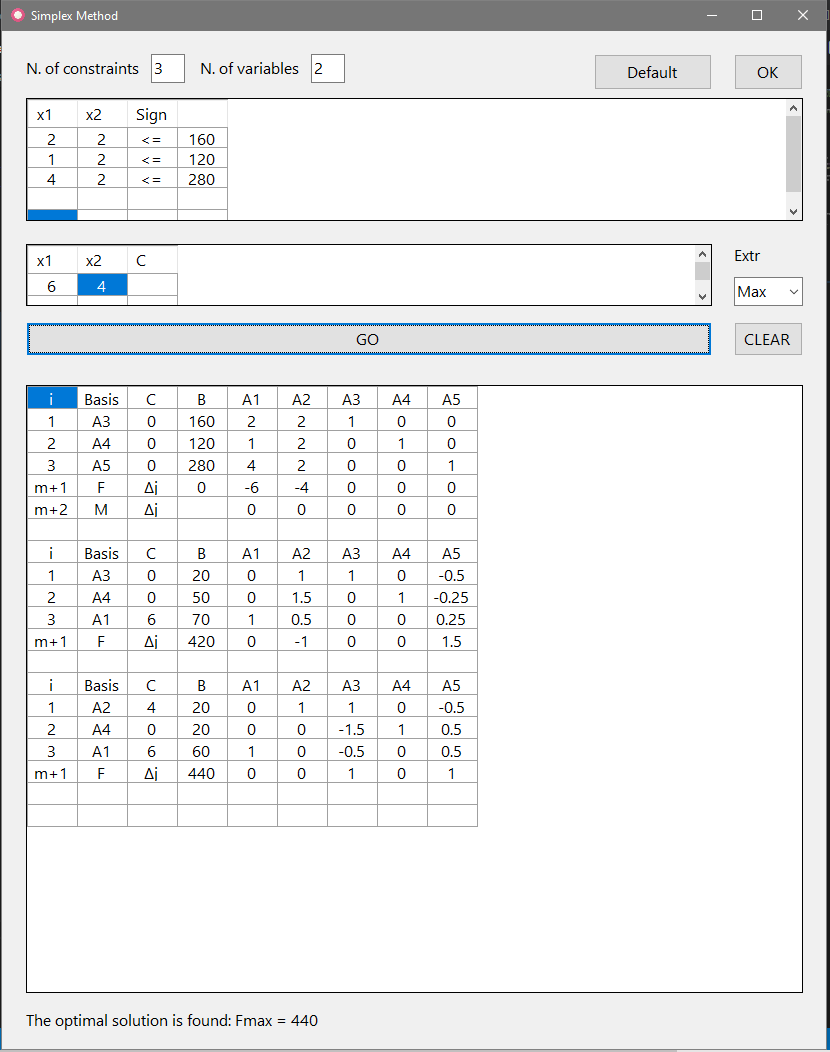
\includegraphics[width=12cm]{tarea3.PNG}
        \caption{Resolución de la tarea 3 en C\#.}
    \end{figure}
    \subsection{Tarea 4}
    \subsubsection{Problema 1}
    \begin{figure}[H]
        \[\begin{matrix}
            F\!.\!O:&\text{Max (z)}:&50x+80y\\
            S.\!a: &&x+y\leq 100\\
            &&x\leq 250\\
            &&y\leq 250\\
            &&x-2y=0\\
            &&x,\, y\geq 0
        \end{matrix}\]
        \caption{Modelo del Problema 1.}
    \end{figure}
    \begin{figure}[H]
        \centering
        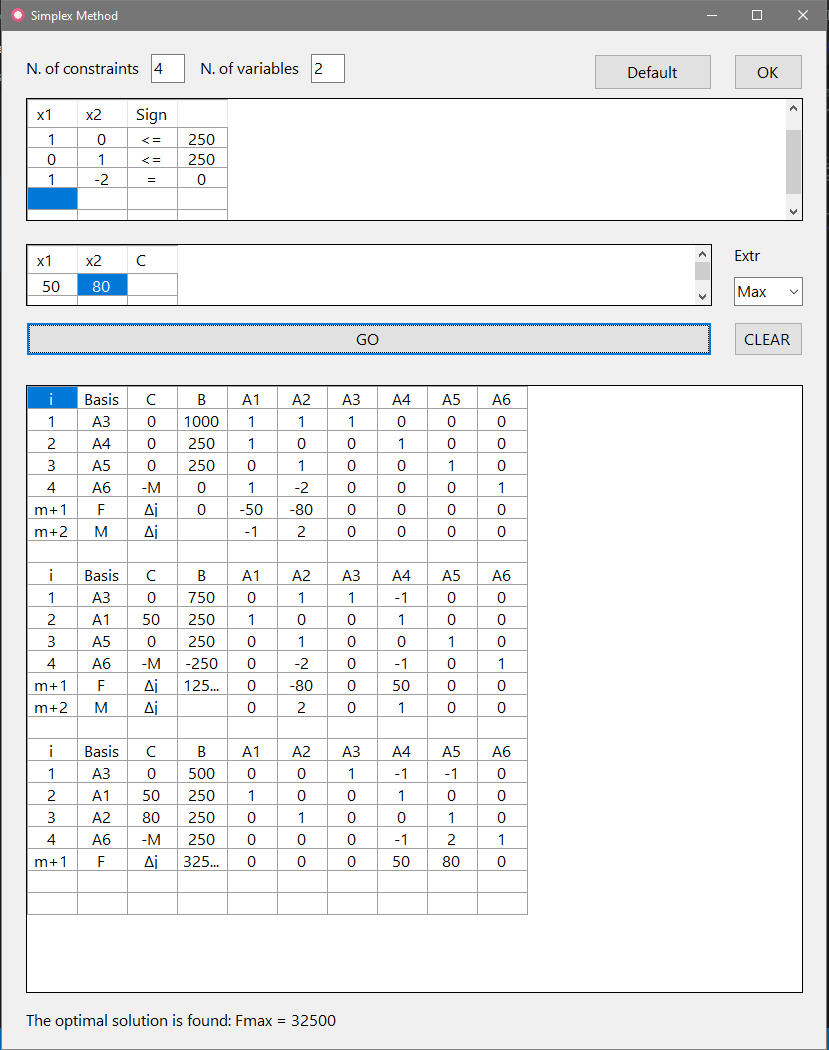
\includegraphics[width=12cm]{problema1.PNG}
        \caption{Resolución del Problema 1 en C\#.}
    \end{figure}
    \subsubsection{Problema 2}
    \begin{figure}[H]
        \[\begin{matrix}
            F\!.\!O:&\text{Max (z)}:&0.4x+1.4y\\
            S.\!a: &&0.6x+0.45y\leq 8100\\
            &&0.15x+0.3y\leq 3000\\
            &&x,\, y\geq 0
        \end{matrix}\]
        \caption{Modelo del Problema 2.}
    \end{figure}
    \begin{figure}[H]
        \centering
        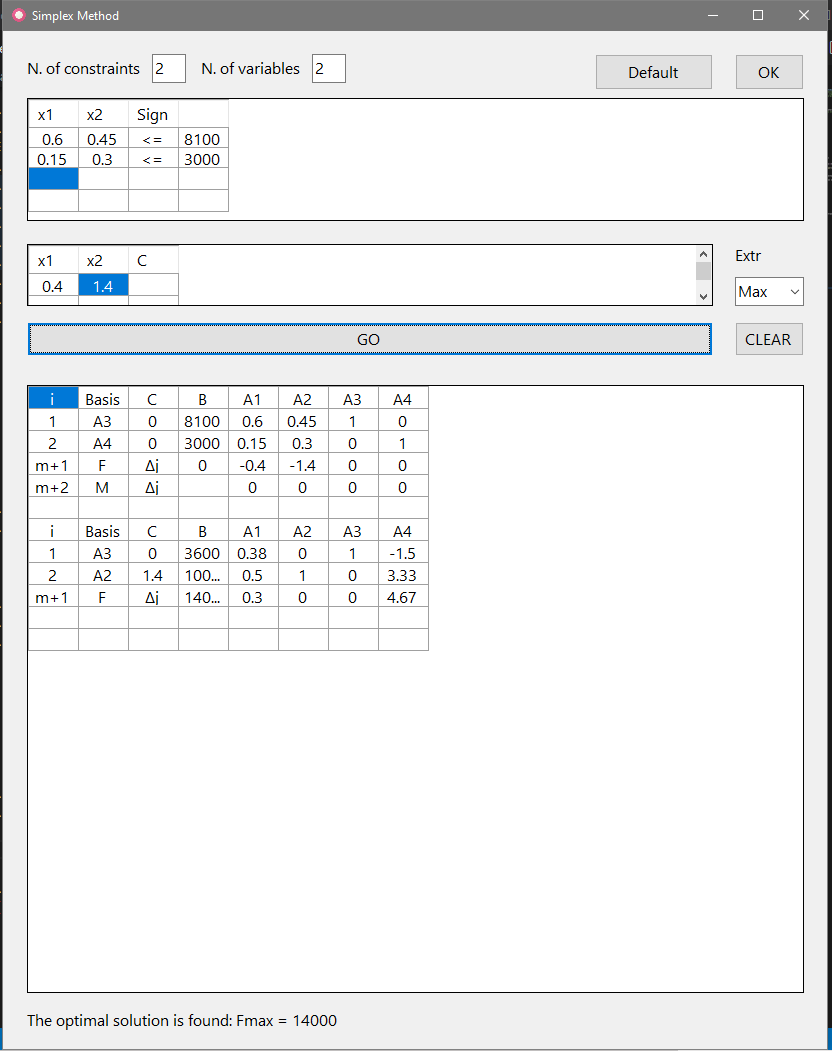
\includegraphics[width=12cm]{problema2.PNG}
        \caption{Resolución del Problema 2 en C\#.}
    \end{figure}
    \section{Unidad 2}
    \subsection{Actividad del 20 de octubre del 2020}
    \begin{figure}[H]
        \[\begin{matrix}
            &D1&D2&D3&D4&D5&\text{Oferta}\\
          O1&13&10&22&29&18&50\\
          O2&14&13&16&21&11&60\\
          O3&3&0&5&11&6&70\\
          O4&18&4&19&23&11&40\\
          O5&30&24&34&36&28&30\\
          \text{Demanda}&30&50&40&50&60
        \end{matrix}\]
        \caption{Modelo de la actividad del 20 de octubre del 2020.}
    \end{figure}
    \begin{figure}[H]
        \centering
        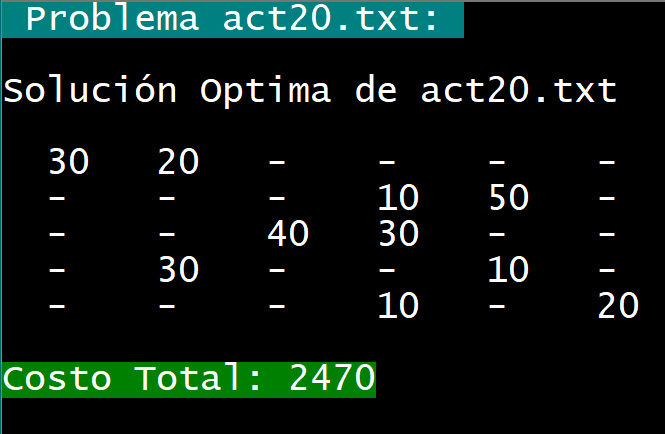
\includegraphics[width=8cm]{act20.PNG}
        \caption{Resolución de la actividad del 20 de octubre del 2020 en C\#.}
    \end{figure}
    \subsection{Actividad del 27 de octubre del 2020}
    \begin{figure}[H]
        \[\begin{matrix}
            &D1&D2&D3&D4&\text{Oferta}\\
        O1&5&8&6&5&40\\
        O2&7&4&7&3&50\\
        O3&4&5&4&6&30\\
        \text{Demanda}&30&20&30&40
        \end{matrix}\]
        \caption{Modelo de la actividad del 27 de octubre del 2020.}
    \end{figure}
    \begin{figure}[H]
        \centering
        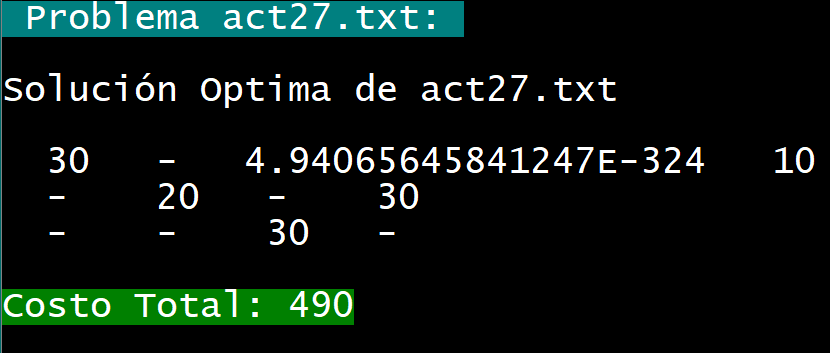
\includegraphics[width=8cm]{act27.PNG}
        \caption{Resolución de la actividad del 27 de octubre del 2020 en C\#.}
    \end{figure}
    \subsection{Actividad del 29 de octubre del 2020}
    \begin{figure}[H]
        \[\begin{matrix}
            \text{Actividad}&T_o&T_{mp}&T_p\\
            A&1&1&1\\
            B&1&2&3\\
            C&2&3&4\\
            D&2&4&6\\
            E&1&3&5\\
            F&1&2&3\\
            G&0&1&2\\
            H&5&7&9\\
            I&6&8&10\\
            J&5&7&15\\
            K&6&7&8\\
            L&3&5&7\\
            M&1&1&1\\
            N&1&2&3\\
            O&2&3&4\\
            P&1&2&3\\
            Q&1&2&3
        \end{matrix}\]
        \caption{Datos de la Actividad del 29 de octubre del 2020.}
    \end{figure}
    \begin{figure}[H]
        \centering
        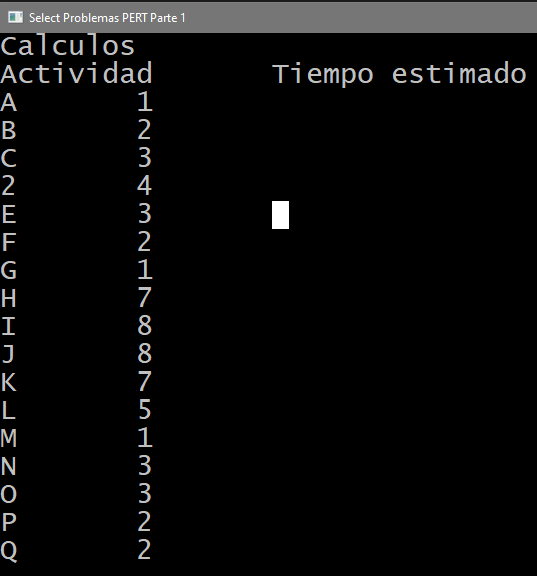
\includegraphics[width=10cm]{act29p1.PNG}
        \caption{Tiempos estimados la Actividad del 29 de octubre del 2020.}
    \end{figure}
    \begin{figure}[H]
        \centering
        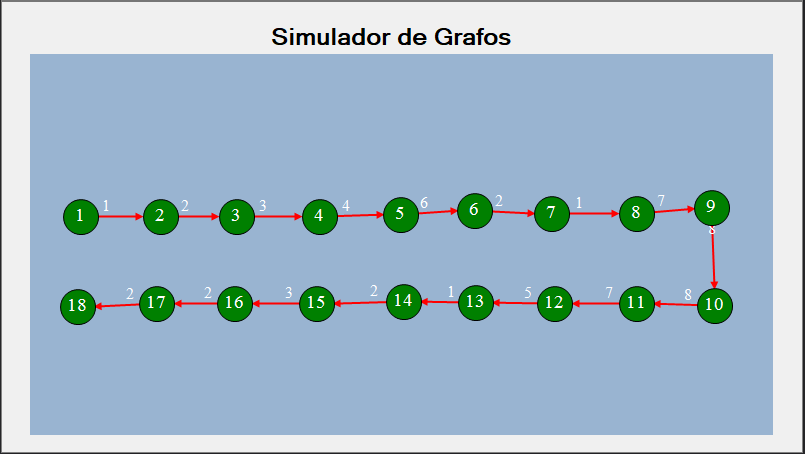
\includegraphics[width=12cm]{act29p2.PNG}
        \caption{Diagrama de Red de la Actividad del 29 de octubre del 2020.}
    \end{figure}
    \subsection{Tarea 1}
    \begin{figure}[H]
        \[\begin{matrix}
            &D1&D2&D3&D4&\text{Oferta}\\
        O1&2&3&4&6&100\\
        O2&1&5&8&3&120\\
        O3&8&5&1&4&80\\
        O4&4&5&6&3&95\\
        \text{Demanda}&125&50&130&90
        \end{matrix}\]
        \caption{Modelo de la tarea 1.}
    \end{figure}
    \begin{figure}[H]
        \centering
        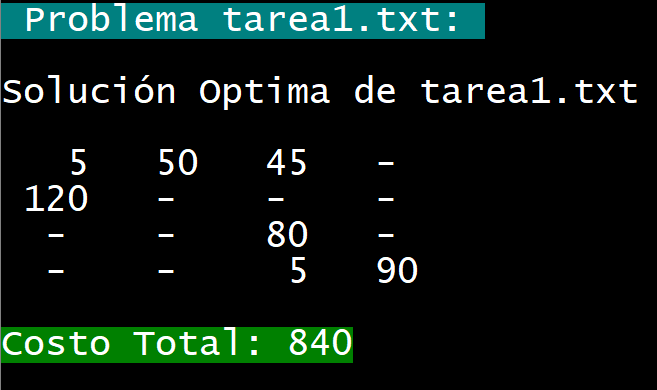
\includegraphics[width=12cm]{tarea1U2.PNG}
        \caption{Resolución de la tarea 1 en C\#.}
    \end{figure}
    \subsection{Tarea 2}
    Se resolvió el mismo problema de la Tarea 1.
    \subsection{Tarea 3}
    \begin{figure}[H]
        \[\begin{matrix}
            &D1&D2&D3&\text{Oferta}\\
        O1&8&12&10&650\\
        O2&10&14&9&650\\
        O3&11&8&12&500\\
        \text{Demanda}&600&800&400
        \end{matrix}\]
        \caption{Modelo de la Tarea 3.}
    \end{figure}
    \begin{figure}[H]
        \centering
        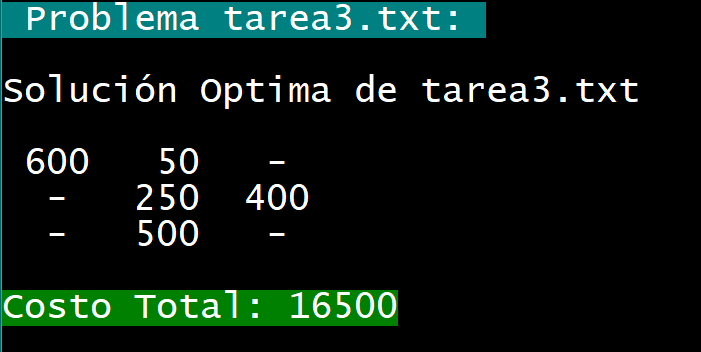
\includegraphics[width=12cm]{tarea3U2.PNG}
        \caption{Resolución de la Tarea 3 en C\#.}
    \end{figure}
    \subsection{Tarea 4}
    \subsubsection{Problema 1}
    \begin{figure}[H]
        \[\begin{matrix}
            \text{Actividad}&\text{Predecesora}\\
            \text{Inicio}&-\\
            A&\text{Inicio}\\
            B&\text{Inicio}\\
            C&B\\
            D&C\\
            E&A\text{ y }D\\
            \text{Fin}&E
        \end{matrix}\]
        \caption{Datos del Problema 1.}
    \end{figure}
    \begin{figure}[H]
        \centering
        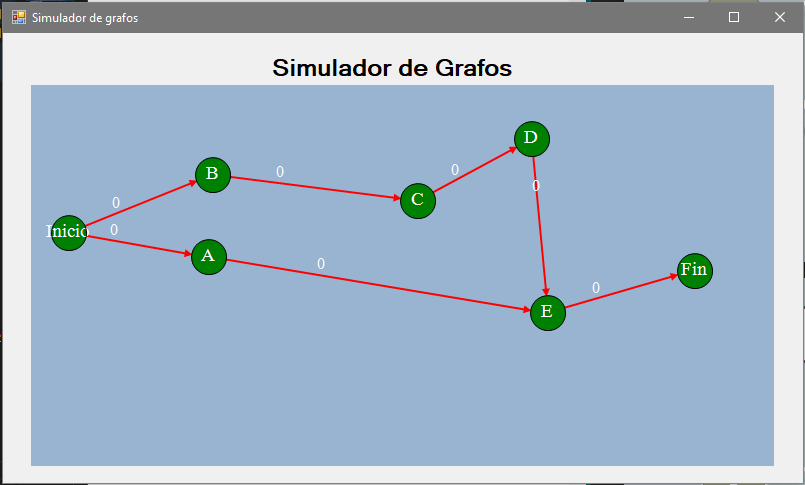
\includegraphics[width=12cm]{tarea4p1.PNG}
        \caption{Resolución del problema 1 de la Tarea 4 en C\#.}
    \end{figure}
    \subsubsection{Problema 2}
    \begin{figure}[H]
        \[\begin{matrix}
            \text{Actividad}&\text{Predecesora}&\text{Tiempo}\\
            A&-&10\\
            B&A&5\\
            C&-&5\\
            D&C&8\\
            E&B\text{ y }D&2\\
            F&E&5\\
            G&F&2
        \end{matrix}\]
        \caption{Datos del Problema 2}
    \end{figure}
    \begin{figure}[H]
        \centering
        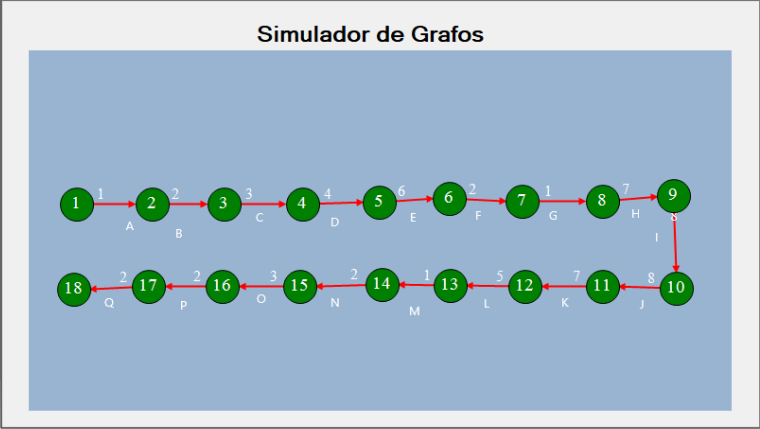
\includegraphics[width=12cm]{tarea4p2.PNG}
        \caption{Resolución del Problema 2 de la Tarea 4 en C\#.}
    \end{figure}
    \subsection{Tarea 5}
    \begin{figure}[H]
        \[\begin{matrix}
            \text{ID}&\text{Tarea}&\text{Descripción}&\text{Predecesor}&\text{TN}\\
            1&A&\text{Preparación del manuscrito (autor)}&&30\\
            2&B&\text{Diseño de materiales promocionales}&1&6\\
            3&C&\text{Producción de materiales promocionales}&2; 7&4\\
            4&D&\text{Corrección del manuscrito}&1&5\\
            5&E&\text{Corrección de galera y revisión}&4&10\\
            6&F&\text{Producción del libro final}&7; 5&8\\
            7&G&\text{Obtención de permisos lega;es y derechos}&1&14\\
            8&H&\text{Captación en ventas}&3; 6&2
        \end{matrix}\]
        \caption{Datos de la Tarea 5.}
    \end{figure}
    \begin{figure}[H]
        \centering
        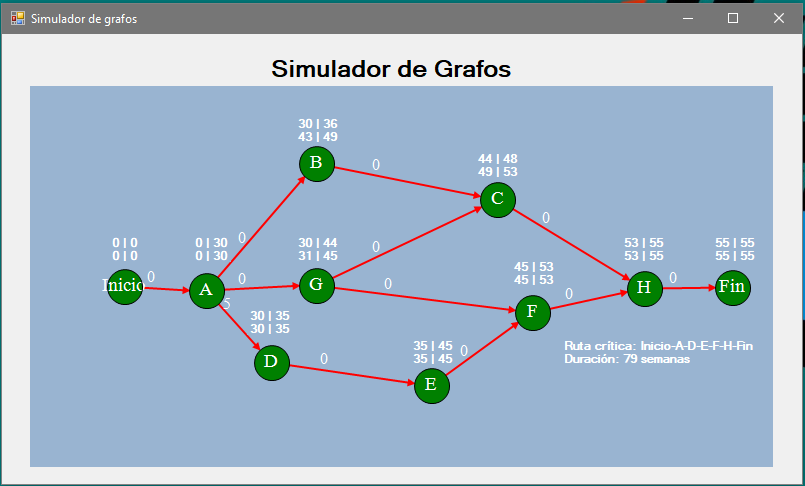
\includegraphics[width=10cm]{TAREA5.PNG}
        \caption{Diagrama de Red de la Tarea 5.}
    \end{figure}
\end{document}